\documentclass{article}
\usepackage{amsmath,amsthm,amssymb,amsfonts}
\usepackage{setspace,enumitem}
\usepackage{graphicx}
\usepackage{hyperref}
\usepackage{natbib}
\usepackage{afterpage}
\usepackage{xcolor}
\usepackage{etoolbox}
\usepackage{booktabs}
\usepackage{pdfpages}
\usepackage{multicol}
\usepackage{geometry}
\usepackage{accents}
\usepackage{bbm}
\usepackage{placeins}
\usepackage{verbatim}
\hypersetup{
	colorlinks,
	linkcolor={blue!90!black},
	citecolor={red!90!black},
	urlcolor={blue!90!black}
}

\newtheorem{theorem}{Theorem}
\newtheorem{assumption}{Assumption}
\newtheorem{definition}{Definition}
\newtheorem{lemma}{Lemma}
\setlength{\parindent}{0cm}
\geometry{margin = 1in}

\newcommand{\R}{\mathbb{R}}
\newcommand{\ubar}[1]{\underaccent{\bar}{#1}}
\newcommand{\Int}{\text{Int}}
\newcommand{\xbf}{\mathbf{x}}
\newcommand{\Abf}{\mathbf{A}}
\newcommand{\Bbf}{\mathbf{B}}
\newcommand{\Gbf}{\mathbf{G}}
\newcommand{\bbf}{\mathbf{b}}
\newcommand{\one}{\mathbbm{1}}

\newtoggle{extended}
\settoggle{extended}{false}

\title{FIN 970: Final Exam}
\author{Alex von Hafften}

\begin{document}

\maketitle

\section{Problem 1a: Term Structure}

\begin{enumerate}

\item Use SDF approach.

\textbf{Solution:} Conjecture $P_t^n = \exp(A_n + B_n'X_t)$. Proof by induction.

For $n=1$,

\begin{align*}
P_t^1 
&= 
E_t[M_{t+1} \cdot 1]\\
\implies\exp(A_1 + B_1'X_t) 
&= 
E_t \Bigg[ \exp \Bigg(-\delta_0 - \delta_1 X_t - \frac{1}{2} \lambda_t'\lambda_t - \lambda_t' \varepsilon_{t+1}\Bigg) \Bigg]\\
\implies E_t \Bigg[ -\delta_0 - \delta_1 X_t - \frac{1}{2} \lambda_t'\lambda_t - \lambda_t' \varepsilon_{t+1} \Bigg]
&= -\delta_0 -\delta_1 X_t - \frac{1}{2}\lambda_t'\lambda_t \\
Var_t\Bigg[ -\delta_0 - \delta_1 X_t - \frac{1}{2} \lambda_t'\lambda_t - \lambda_t' \varepsilon_{t+1} \Bigg]
&= \lambda_t'\lambda_t\\
\implies
\exp(A_1 + B_1'X_t) 
&= 
\exp (-\delta_0 - \delta_1 X_t ) \\
\implies
\begin{cases}
A_1 = -\delta_0\\
B_1 = -\delta_1'
\end{cases}
\end{align*}

For some $n>1$, the Euler equation holds:

\begin{align*}
P_t^n &= E_t[M_{t+1} P_{t+1}^{n-1}]\\
\exp(A_{n} + B_{n}'X_{t})
&= E_t \Bigg[\exp \Bigg(-r_t - \frac{1}{2} \lambda_t'\lambda_t - \lambda_t' \varepsilon_{t+1}\Bigg) \exp(A_{n-1} + B_{n-1}'X_{t+1})\Bigg]\\
&= E_t \Bigg[\exp \Bigg(-\delta_0 - \delta_1 X_t - \frac{1}{2} \lambda_t'\lambda_t - \lambda_t' \varepsilon_{t+1} + A_{n-1} + B_{n-1}'(\mu + \Phi X_t + \Sigma \varepsilon_{t+1} ) \Bigg)\Bigg]\\
&= E_t \Bigg[\exp \Bigg(-\delta_0 - \delta_1 X_t - \frac{1}{2} \lambda_t'\lambda_t  + A_{n-1} + B_{n-1}'\mu + B_{n-1}'\Phi X_t + [B_{n-1}'\Sigma - \lambda_t'] \varepsilon_{t+1}  \Bigg)\Bigg]
\end{align*}

\begin{align*}
& E_t \Bigg[-\delta_0 - \delta_1 X_t - \frac{1}{2} \lambda_t'\lambda_t  + A_{n-1} + B_{n-1}'\mu + B_{n-1}'\Phi X_t + [B_{n-1}'\Sigma - \lambda_t'] \varepsilon_{t+1}  \Bigg] \\
&=  -\delta_0 - \delta_1 X_t - \frac{1}{2} \lambda_t'\lambda_t  + A_{n-1} + B_{n-1}'\mu + B_{n-1}'\Phi X_t\\
& Var_t\Bigg[-\delta_0 - \delta_1 X_t - \frac{1}{2} \lambda_t'\lambda_t  + A_{n-1} + B_{n-1}'\mu + B_{n-1}'\Phi X_t + [B_{n-1}'\Sigma - \lambda_t'] \varepsilon_{t+1}  \Bigg] \\
&= [B_{n-1}'\Sigma - \lambda_t'][B_{n-1}'\Sigma - \lambda_t']'\\
&= B_{n-1}'\Sigma \Sigma' B_{n-1} + \lambda_t' \lambda_t - 2 B_{n-1}'\Sigma \lambda_t
\end{align*}

\begin{align*}
\exp(A_{n} + B_{n}'X_{t})
&= \exp\Bigg(-\delta_0 - \delta_1 X_t - \frac{1}{2} \lambda_t'\lambda_t  + A_{n-1} + B_{n-1}'\mu + B_{n-1}'\Phi X_t \\&+ \frac{1}{2} B_{n-1}'\Sigma \Sigma' B_{n-1} + \frac{1}{2}\lambda_t' \lambda_t - B_n'\Sigma (\lambda_0 + \lambda_1 X_t) \Bigg)\\
&= \exp\Bigg(-\delta_0   + A_{n-1} + B_{n-1}'\mu - B_{n-1}'\Sigma \lambda_0 + \frac{1}{2} B_{n-1}'\Sigma \Sigma' B_{n-1}+ (- \delta_1  + B_{n-1}'\Phi - B_{n-1}'\Sigma \lambda_1 )X_t  ) \Bigg)\\
\implies
&
\begin{cases}
A_n = - \delta_0 + A_{n-1} + B_{n-1}'(\mu - \Sigma \lambda_0) + \frac{1}{2} B_{n-1}'\Sigma \Sigma' B_{n-1}\\
B_n = - \delta_1  + (\Phi - \Sigma \lambda_1)' B_{n-1}
\end{cases}
\end{align*}

\item Use risk-neutral density approach.

\textbf{Solution:} Conjecture $P_t^n = \exp(C_n + D_n'X_t)$. Proof by induction.

For $n=0$,

\begin{align*}
P_t^1 
&= 
e^{-r_t}E_t^Q[1]\\
\exp(C_1 + D_1'X_t) 
&= 
\exp (-\delta_0 - \delta_1 X_t) \\
\implies&
\begin{cases}
C_1 = -\delta_0\\
D_1 = -\delta_1'
\end{cases}
\end{align*}

For some $n>1$, the Euler equation holds:

\begin{align*}
P_t^n 
&= e^{-r_t} E_t^Q [P_{t+1}^{n-1}]\\
\exp(C_n + D_n'X_t)
&= e^{-r_t} E_t^Q [\exp(C_{n-1} + D_{n-1}'X_{t+1})]\\
&= e^{-r_t} E_t^Q [\exp(C_{n-1} + D_{n-1}'(\mu^Q + \Phi^Q X_t + \Sigma \varepsilon_{t+1}^Q))]\\
&= e^{-r_t} E_t^Q [\exp(C_{n-1} + D_{n-1}'\mu^Q + D_{n-1}'\Phi^Q X_t + D_{n-1}'\Sigma \varepsilon_{t+1}^Q)]
\end{align*}

\begin{align*}
E_t^Q[C_{n-1} + D_{n-1}'\mu^Q + D_{n-1}'\Phi^Q X_t + D_{n-1}'\Sigma \varepsilon_{t+1}^Q] 
&= E_t[C_{n-1} + D_{n-1}'\mu^Q + D_{n-1}'\Phi^Q X_t]\\
Var_t^Q [C_{n-1} + D_{n-1}'\mu^Q + D_{n-1}'\Phi^Q X_t + D_{n-1}'\Sigma \varepsilon_{t+1}^Q]
&= D'_{n-1} \Sigma \Sigma' D_{n-1}
\end{align*}

\begin{align*}
\exp(C_n + D_n'X_t)
&=  \exp \Bigg(-\delta_0 - \delta_1 X_t + C_{n-1} + D_{n-1}'\mu^Q + D_{n-1}'\Phi^Q X_t + \frac{1}{2} D'_{n-1} \Sigma \Sigma' D_{n-1} \Bigg)\\
& \begin{cases}
C_n = -\delta_0  + C_{n-1} + D_{n-1}'\mu^Q  + \frac{1}{2} D'_{n-1} \Sigma \Sigma' D_{n-1}\\
D_n = - \delta_1' + \Phi^{Q'} D_{n-1}
\end{cases}
\end{align*}

\item Show that this is a one-to-one mapping between the risk-neutral parameters $(\mu^Q,  \Phi^Q)$ and the market prices of risk $(\lambda_0, \lambda_1)$.

\bigskip

\textbf{Solution:} Clearly, parts (1) and (2) are equivalent iff

\begin{align*}
\mu^Q &= \mu - \Sigma \lambda_0  \iff \lambda_0 = \Sigma^{-1}(\mu - \mu^Q)\\
\Phi^Q &= \Phi - \Sigma \lambda_1 \iff \lambda_1 = \Sigma^{-1}(\Phi - \Phi^Q)
\end{align*}

with $A_n = C_n$ and $B_n = D_n$. Thus, we can go back and forth from SDF to risk-neutral densities to price bonds of any maturity.

\bigskip



\end{enumerate}

\pagebreak

\section{Problem 2h - LRR Model}

\begin{enumerate}

\item Conjecture $pc_t$ is linear in state variables. Solve for $pc_t$ and $r_{c,t+1}$. Explain how risk exposures depend on preferences and consumption dynamics.

\bigskip

\textbf{Solutions:} Conjecture that $pc_t = A_0 + A_x x_t$. 
Using the Campbell-Schiller approximation to log-linearization the consumption return:

\begin{align*}
R_{C,t+1} 
&= \frac{P_{C,t+1} + C_{t+1}}{P_{C,t}} \\
&=  \frac{\frac{P_{C,t+1}}{C_{t+1}} + 1}{\frac{P_{C,t}}{C_t}} \frac{C_{t+1}}{C_{t}}\\
r_{c,t+1} 
&= \log(\exp(pc_{t+1}) +1) - pc_t +\Delta c_{t+1} \\
&\approx \Bigg[\log(\exp(\bar{pc}) +1) + \frac{\exp(\bar{pc})}{\exp(\bar{pc}) + 1} (pc_{t+1} - \bar{pc})\Bigg]- pc_t +\Delta c_{t+1} \\
&= \underbrace{\log(\exp(\bar{pc}) +1)- \frac{\exp(\bar{pc})}{\exp(\bar{pc}) + 1} \bar{pc}}_{\equiv \kappa_0} + \underbrace{\frac{\exp(\bar{pc})}{\exp(\bar{pc}) + 1}}_{\equiv \kappa_1} pc_{t+1} - pc_t +\Delta c_{t+1} 
\end{align*}

where $pc_t = \log(P_{C,t}/C_{t})$. Alternatively, we can express the return in terms of the demeaned price-consumption ratio,

\begin{align*}
r_{c, t+1} 
&= \kappa_0 + \kappa_1 pc_{t+1} - pc_t + \Delta c_{t+1}\\
&= -\log \kappa_1 + \kappa_1 \underbrace{\tilde{pc}_{t+1}}_{\equiv pc_{t+1} - \bar{pc}} - \tilde{pc}_t + \Delta c_{t+1}
\end{align*}

Given the guess for $pc_t$, its unconditional expected value is $\bar{pc} = A_0$, so $\tilde{pc}_t = A_x x_t$. Plugging the dynamics for volatility and consumption:

\begin{align*}
\tilde{pc}_{t+1} 
&= A_x x_{t+1} \\
&= A_x [\rho x_t + \varphi_e \sigma e_{t+1}] \\
&= A_x \rho x_t  + A_x \varphi_e \sigma e_{t+1}  
\end{align*}

Plugging into the consumption return:

\begin{align*}
r_{c, t+1} 
&= -\log \kappa_1 + \kappa_1 \tilde{pc}_{t+1} - \tilde{pc}_t + \Delta c_{t+1}\\
&= -\log \kappa_1 + \kappa_1 [A_x \rho x_t  + A_x \varphi_e \sigma e_{t+1} ] - [A_x x_t] + [\mu + x_t + \sigma \varepsilon_{t+1}] \\
&= [-\log \kappa_1 + \mu] +  [\kappa_1 A_x \rho - A_x + 1] x_t  + \kappa_1 A_x \varphi_e \sigma e_{t+1} + \sigma \varepsilon_{t+1}
\end{align*}


For any asset with return $R_{i,t+1}$, the Euler equation holds and if the return is log-normal:

\begin{align*}
1 &= E_t[M_{t+1} R_{i,t+1}]\\
&= E_t[\exp(m_{t+1} + r_{i,t+1})]\\
&= \exp(E_t[m_{t+1} + r_{i,t+1}] + \frac{1}{2} Var_t[m_{t+1} + r_{i,t+1}])\\
\implies
0&= E_t[m_{t+1} + r_{i,t+1}] + \frac{1}{2} Var_t[m_{t+1} + r_{i,t+1}]
\end{align*}


In particular for the consumption assets, the Euler equation holds. 

\begin{align*}
m_{t+1} + r_{c,t+1} 
&= \theta \log \delta - \frac{\theta}{\psi} \Delta c_{t+1} + \theta r_{c,t+1}\\
&= \theta \log \delta - \frac{\theta}{\psi} [\mu + x_t + \sigma \varepsilon_{t+1}] + \theta [(-\log \kappa_1 + \mu) +  (\kappa_1 A_x \rho - A_x + 1) x_t  + \kappa_1 A_x \varphi_e \sigma e_{t+1} + \sigma \varepsilon_{t+1}]\\
&= 
\Bigg[\theta \log \delta 
- \frac{\theta}{\psi} \mu 
+  \theta (-\log \kappa_1 + \mu) \Bigg]
+  \Bigg[\theta(\kappa_1 A_x \rho - A_x + 1) - \frac{\theta}{\psi}\Bigg] x_t  
+ \theta\Bigg[1 - \frac{1}{\psi}  \Bigg]\sigma\varepsilon_{t+1} 
+ \theta\kappa_1 A_x \varphi_e \sigma e_{t+1}
\end{align*}

The expected value and variance of $m_{t+1} + r_{c,t+1}$ is

\begin{align*}
E_t[m_{t+1} + r_{c,t+1}] 
&= \Bigg[\theta \log \delta 
- \frac{\theta}{\psi} \mu 
+  \theta (-\log \kappa_1 + \mu) \Bigg]
+  \Bigg[\theta(\kappa_1 A_x \rho - A_x + 1) - \frac{\theta}{\psi}\Bigg] x_t \\
Var_t[m_{t+1} + r_{c,t+1}]
&= \theta^2 \Bigg[1 - \frac{1}{\psi}  \Bigg]^2\sigma^2 
+ \theta^2 \kappa_1^2 A_x^2 \varphi_e^2 \sigma^2
\end{align*}

Thus, we can plug the expected value and variance back in:

\begin{align*}
0&= E_t[m_{t+1} + r_{i,t+1}] + \frac{1}{2} Var_t[m_{t+1} + r_{i,t+1}]\\
\implies
0 &= \Bigg[\theta \log \delta 
- \frac{\theta}{\psi} \mu 
+  \theta (-\log \kappa_1 + \mu) \Bigg]
+  \Bigg[\theta(\kappa_1 A_x \rho - A_x + 1) - \frac{\theta}{\psi}\Bigg] x_t 
+ \frac{1}{2} \theta^2 \Bigg[1 - \frac{1}{\psi}  \Bigg]^2\sigma^2 
+ \frac{1}{2} \theta^2 \kappa_1^2 A_x^2 \varphi_e^2 \sigma^2 \\
\implies &
\begin{cases}
0 &=\Bigg[\theta \log \delta 
- \frac{\theta}{\psi} \mu 
+  \theta (-\log \kappa_1 + \mu) \Bigg]
+ \frac{1}{2} \theta^2 \Bigg[1 - \frac{1}{\psi}  \Bigg]^2\sigma^2 
+ \frac{1}{2} \theta^2 \kappa_1^2 A_x^2 \varphi_e^2 \sigma^2 \\
0 &=  \Bigg[\theta(\kappa_1 A_x \rho - A_x + 1) - \frac{\theta}{\psi}\Bigg]
\end{cases}\\
\implies
A_x &= \frac{1 - 1/\psi}{1 - \kappa_1 \rho}
\end{align*}


Thus, asset valuations respond positive to expected growth if 

\begin{align*}
A_x > 0
\iff 
\frac{1 - 1/\psi}{1 - \kappa_1 \rho} > 0 
\iff
1 > 1/\psi 
\iff
\psi > 1
\end{align*}

Economically, this parameter restriction means that the substitution effect dominates the wealth effect.

Using the solution for $A_x$, we can express $r_{c,t+1}$ as 

\begin{align*}
r_{c,t+1} &= [-\log \kappa_1 + \mu] +  [\kappa_1 A_x \rho - A_x + 1] x_t  + \kappa_1 A_x \varphi_e \sigma e_{t+1} + \sigma \varepsilon_{t+1}\\
&= [-\log \kappa_1 + \mu] +  \frac{1}{\psi} x_t  + \frac{(1-1/\psi)\kappa_1 \varphi_e }{1- \kappa_1 \rho} \sigma e_{t+1} + \sigma \varepsilon_{t+1}\\
&= r_{c,0} +  \frac{1}{\psi} x_t  + B_x \varphi_e\sigma e_{t+1} + B_c \sigma \varepsilon_{t+1}
\end{align*}

where $r_{c,0} \equiv -\log \kappa_1 + \mu$, $B_x \equiv \frac{(1-1/\psi)\kappa_1 }{1- \kappa_1 \rho}$, and $B_c \equiv 1$.

\pagebreak

\item Solve for $M_{t+1}$.

\bigskip

\textbf{Solution:} 

\begin{align*}
m_{t+1} 
&= \theta \log \delta - \frac{\theta}{\psi} \Delta c_{t+1} + (\theta - 1)r_{c,t+1}\\
&= \theta \log \delta - \frac{\theta}{\psi} \Bigg[\mu + x_t + \sigma \varepsilon_{t+1} \Bigg] + (\theta - 1)\Bigg[r_{c,0} +  \frac{1}{\psi} x_t  + B_x \varphi_e \sigma e_{t+1} + B_c \sigma \varepsilon_{t+1}\Bigg]\\
&= \Bigg[\theta \log \delta - \frac{\theta}{\psi} \mu + (\theta - 1) r_{c,0}\Bigg]
+ \Bigg[-\frac{\theta}{\psi} + \frac{\theta - 1}{\psi} \Bigg] x_t
+ (\theta - 1)B_x \varphi_e \sigma e_{t+1}
+ (-\theta/\psi + (\theta - 1)B_c) \sigma \varepsilon_{t+1}\\
&= m_0 - m_x x_t -\lambda_x \varphi_e \sigma e_{t+1} - \lambda_c \sigma \varepsilon_{t+1}
\end{align*}

where

\begin{align*}
m_0 &\equiv \Bigg[\theta \log \delta - \frac{\theta}{\psi} \mu + (\theta - 1) r_{c,0}\Bigg]\\
m_x &\equiv -1/\psi \\
\lambda_x 
&\equiv (1 - \theta) B_x\\
&= (1 - \theta )\frac{(1-1/\psi)\kappa_1 }{1- \kappa_1 \rho}\\
\lambda_c 
&\equiv \theta/\psi - \theta + 1 \\
&= - \gamma
\end{align*}

If $\psi > 1 \implies \lambda_x > 0$ and $\lambda_c < 0$ by assumption.

\bigskip

\item Consumption strip at maturity $n = 1$.

\bigskip

\textbf{Solution:}

\begin{align*}
P_{t,1} &= E_t[M_{t+1} C_{t+1}]\\
\implies
\frac{P_{t,1}}{C_t} &= E_t \Bigg[M_{t+1} \frac{C_{t+1}}{C_t} \Bigg]\\
&= E_t [\exp(m_{t+1} + \Delta c_{t+1} ) ]\\
&= \exp(E_t [m_{t+1} + \Delta c_{t+1} ] + \frac{1}{2} V_t[m_{t+1} + \Delta c_{t+1} ])\\
\implies
pc_{t,1} &= E_t [m_{t+1} + \Delta c_{t+1} ] + \frac{1}{2} V_t[m_{t+1} + \Delta c_{t+1} ] \\
\implies
m_{t+1} + \Delta c_{t+1} 
&= m_0 - m_x x_t -\lambda_x \varphi_e \sigma e_{t+1} - \lambda_c \sigma \varepsilon_{t+1} + \mu + x_t + \sigma \varepsilon_{t+1}\\
&= m_0 + \mu - (m_x -1)x_t -\lambda_x \varphi_e \sigma e_{t+1} - (\lambda_c - 1) \sigma \varepsilon_{t+1}\\
\implies
E_t [m_{t+1} + \Delta c_{t+1} ] 
&= m_0 + \mu - (m_x -1)x_t \\
\implies
V_t [m_{t+1} + \Delta c_{t+1} ]
&=\lambda_x^2 \varphi_e^2 \sigma^2 + (\lambda_c - 1)^2 \sigma^2 \\
pc_{t,1} &= m_0 + \mu + (1 - m_x)x_t + \frac{1}{2} \lambda_x^2 \varphi_e^2 \sigma^2 + \frac{1}{2}(\lambda_c - 1)^2 \sigma^2 
\end{align*}

\pagebreak

\item Solve for the return on the consumption strip and risk premium

\bigskip

\textbf{Solution:} The return on the consumption strip is:

\begin{align*}
\log r_{t+1,1} 
&= \Delta c_{t+1} - pc_{t,1} \\
&= \mu + x_t + \sigma \varepsilon_{t+1} - m_0 - \mu - (1 - m_x)x_t - \frac{1}{2} \lambda_x^2 \varphi_e^2 \sigma^2 - \frac{1}{2}(\lambda_c - 1)^2 \sigma^2\\
&=  - m_0 + m_x x_t + \sigma \varepsilon_{t+1}  - \frac{1}{2} \lambda_x^2 \varphi_e^2 \sigma^2 - \frac{1}{2}(\lambda_c - 1)^2 \sigma^2
\end{align*}

The risk premium of the consumption strip is

\begin{align*}
-Cov_t(r_{t+1, 1}, m_{t+1}) 
&= -Cov_t(- m_0 + m_x x_t + \sigma \varepsilon_{t+1}  - \frac{1}{2} \lambda_x^2 \varphi_e^2 \sigma^2 - \frac{1}{2}(\lambda_c - 1)^2 \sigma^2, \\& m_0 - m_x x_t -\lambda_x \varphi_e \sigma e_{t+1} - \lambda_c \sigma \varepsilon_{t+1})\\
&= -Cov_t( \sigma \varepsilon_{t+1}  , -\lambda_x \varphi_e \sigma e_{t+1} - \lambda_c \sigma \varepsilon_{t+1}) \\
&= \lambda_c \sigma^2 \\
&= -\gamma \sigma^2
\end{align*}

The risk premium on the consumption claim is

\begin{align*}
-Cov_t(r_{c,t+1}, m_{t+1}) 
&= -Cov_t(r_{c,0} +  \frac{1}{\psi} x_t  + B_x \varphi_e\sigma e_{t+1} + B_c \sigma \varepsilon_{t+1}, m_0 - m_x x_t -\lambda_x \varphi_e \sigma e_{t+1} - \lambda_c \sigma \varepsilon_{t+1})\\
&= -Cov_t( B_x \varphi_e\sigma e_{t+1} + B_c \sigma \varepsilon_{t+1}, -\lambda_x \varphi_e \sigma e_{t+1} - \lambda_c \sigma \varepsilon_{t+1})\\
&= B_x\lambda_x \varphi_e^2 \sigma^2 + B_c \lambda_c \sigma^2\\
&= (1-\theta)B_x^2 \varphi_e^2\sigma^2 -\gamma \sigma^2
\end{align*}

The consumption strip has a negative risk premium and the consumption claim has a higher risk premium, so this model is inconsistent with the evidence that short-term consumptions strips have higher average excess returns than claim on all future cash-flows.

\begin{align*}
-Cov_t(r_{t+1, 1}, m_{t+1}) &< -Cov_t(r_{c,t+1}, m_{t+1}) \\
\iff
-\gamma \sigma^2 &< (1-\theta)B_x^2 \varphi_e^2\sigma^2 -\gamma \sigma^2\\
\iff
0 &< (1-\theta)B_x^2 \varphi_e^2\sigma^2
\end{align*}

\item Time-varying risk premium on consumption strips.

\bigskip

\textbf{Solution:} No, this model implies a constant risk premium on consumption strips.  We can introduce time-varying volatility $\sigma_t$. With time-varying volatility, the risk premium of the consumption strip would be $-\gamma \sigma_t^2$, which would vary over time.

\end{enumerate}

\pagebreak

\section{Problem 3}


\pagebreak

\section{Problem 4 - Jumps}

\begin{enumerate}

\item Show that $E_t[Q_{c,t+1}] = E_t[Q_{x,t+1}] = 0$. Sketch typical timeseries.

\textbf{Solution:}

\begin{align*}
E_t[Q_{c,t+1}] 
&= E_t \Bigg[ \sum_{i=1}^{N_{c,t+1}} J_{i,c,t+1} - \lambda_c \mu_{jc} \Bigg]\\
&= E_t \Bigg[E_t \Bigg[ \sum_{i=1}^{N_{c,t+1}} J_{i,c,t+1}\Bigg| N_{c,t+1}\Bigg]\Bigg] - \lambda_c \mu_{jc} \\
&= E_t \Bigg[\sum_{i=1}^{N_{c,t+1}} E_t [ J_{i,c,t+1}| N_{c,t+1}]\Bigg] - \lambda_c \mu_{jc} \\
&= E_t \Bigg[\sum_{i=1}^{N_{c,t+1}} E_t [ J_{i,c,t+1}]\Bigg] - \lambda_c \mu_{jc} \\
&= E_t \Bigg[\sum_{i=1}^{N_{c,t+1}} \mu_{jc}\Bigg] - \lambda_c \mu_{jc} \\
&= \mu_{jc}E_t \Bigg[\sum_{i=1}^{N_{c,t+1}}1 \Bigg] - \lambda_c \mu_{jc} \\
&= \mu_{jc}E_t[N_{c,t+1} ] - \lambda_c \mu_{jc} \\
&= \mu_{jc} \lambda_c - \lambda_c \mu_{jc} \\
&= 0
\end{align*}

Similar argument holds for $E_t[Q_{x,t+1}]$.  

\bigskip

Consider $Q_{c,t+1}] =\sum_{i=1}^{N_{c,t+1}} J_{i,c,t+1} - \lambda_c \mu_{jc}$. During jump times, the first term dominates the second term, so $Q$ is discontinuously negative.  During nonjump times, the first term is zero, so the shock is just $- \lambda_c \mu_{jc}$.  Notice that it is deterministic, constant over time, and positive (since $\mu_{jc} < 0$ by assumption and $\lambda_c > 0$ by definition).  

\bigskip

Thus, a typical time-series looks like the graphs on the following page.  I simulated this series with a $\lambda = 0.1$, $\mu = -1$, and a degenerate jump size distribution, $J_{i,c,t+1} = \mu$ $\forall i, t$.  During nonjump times, $Q$ is small and positive $-\mu\lambda = 0.1$.  With my choice of $\lambda$, my simulation returned only jumps of size one and two.  Size one jumps are $\mu - \mu \lambda = -1 + 0.1 = -0.9$ and size two jumps are $2\mu - \mu \lambda = -2 + 0.1 = -1.9$. In the second figure, I cumulatively adding up the realizations of $Q$.  The series slowly increases during nonjump periods and sharply decreases during jump periods.

\begin{center}
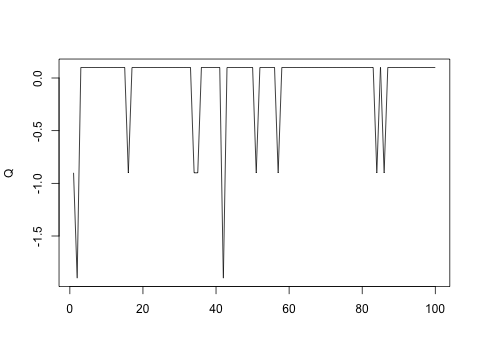
\includegraphics[scale = 0.75]{p4_1}
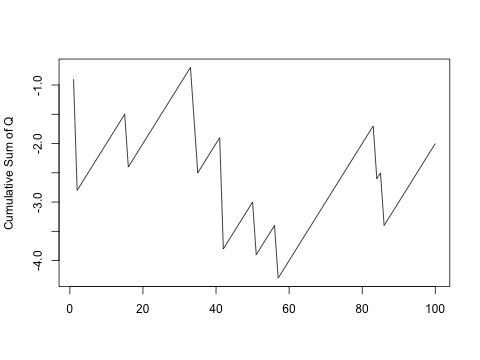
\includegraphics[scale = 0.75]{p4_2}
\end{center}

\pagebreak

\item Recursive utility environment. Solve for the equilibrium stochastic discount factor. Show that the jumps in realized and expected consumption growth are priced. Specifically, show that under the typical assumptions for the preference parameters the market prices of both jump risks are positive. Show that the market price of expected consumption jumps increases in the persistence of the expected consumption growth.

\textbf{Solution:} Recursive preferences are as follows:

$$
U_t = \Bigg[ (1-\delta) C_t^{1-1/\psi} + \delta (E_t U_{t+1}^{1-\gamma})^{\frac{1 - 1/\psi}{1- \gamma}} \Bigg]^{\frac{1}{1-1/\psi}}
$$

They imply the following SDF:

$$
m_{t+1} = \theta \log \delta - \frac{\theta}{\psi} \Delta c_{t+1} + (\theta - 1) r_{c,t+1}
$$

where $\Delta c_{t+1}$ is change in log consumption, $r_{c,t+1}$ is the return on the consumption assets, and $\theta \equiv \frac{1-\gamma}{1-1/\psi}$. Using Campbell-Schiller return log-linearization, we can approximate $r_{c,t+1}$ as

$$
r_{c,t+1} \approx - \log \kappa_1 + \kappa_1 \tilde pc_{t+1} + \Delta c_{t+1} - \tilde pc_t
$$

where $\kappa_1 = \frac{\exp(\bar{pc})}{\exp(\bar{pc}) + 1}$, $\tilde pc_t = pc_t - \bar{pc}$ and $pc_t$ is the log price consumption ratio.  Guess that $pc_t = A_0 + A_x x_t$, then $\tilde pc_t = A_x x_t$ and 

$$
\tilde pc_{t+1} = A_x \rho x_t + A_x\varphi_e \sigma \varepsilon_{t+1} + A_x Q_{x,t+1}
$$

Plugging into the return on consumption asset

\begin{align*}
r_{c,t+1} 
&= -\log \kappa_1 + \kappa_1 [A_x \rho x_t + A_x\varphi_e \sigma \varepsilon_{t+1} + A_x Q_{x,t+1}] + [\mu + x_t + \sigma \eta_{t+1} + Q_{c,t+1}] - A_x x_t\\
&= [-\log \kappa_1 + \mu] + [\kappa_1 A_x \rho  + 1 - A_x] x_t + \kappa_1 A_x \varphi_e \sigma \varepsilon_{t+1} + \sigma \eta_{t+1} + \kappa_1 A_x Q_{x,t+1} + Q_{c,t+1}
\end{align*}

Thus, the SDF plus consumption return is

\begin{align*}
m_{t+1} + r_{c,t+1}
&= \theta \log \delta - \frac{\theta}{\psi} [\mu + x_t + \sigma \eta_{t+1} + Q_{c,t+1}] \\
&+ \theta ([\log \kappa_1 + \mu] + [\kappa_1 A_x \rho  + 1 - A_x] x_t + \kappa_1 A_x \varphi_e \sigma \varepsilon_{t+1} + \sigma \eta_{t+1} + \kappa_1 A_x Q_{x,t+1} + Q_{c,t+1})\\
&= \theta[ \log \delta + (1-1/\psi)\mu - \log \kappa_1]
+ \theta [\kappa_1 A_x \rho  + 1 - A_x - 1/\psi] x_t \\
&+ \theta  \kappa_1 A_x \varphi_e \sigma \varepsilon_{t+1}
+ \theta (1-1/\psi) \sigma \eta_{t+1}
+ \theta \kappa_1 A_x Q_{x,t+1} 
+ \theta (1- 1/\psi) Q_{c,t+1}
\end{align*}


By the Euler equation for any traded asset, $E_t[M_{t+1} R_{i,t+1}] = 1$.

\begin{align*}
& \theta[ \log \delta + (1-1/\psi)\mu - \log \kappa_1]
+ \theta [\kappa_1 A_x \rho  + 1 - A_x - 1/\psi] x_t \\
&+ \frac{1}{2}\theta^2  \kappa_1^2 A_x^2 \varphi_e^2 \sigma^2
+ \frac{1}{2}\theta^2 (1-1/\psi)^2 \sigma^2 \\&
+ \lambda_x[\alpha_x(\theta \kappa_1 A_x)- \theta \kappa_1 A_x \mu_{jx} - 1]
+ \lambda_c[\alpha_c(\theta (1- 1/\psi)) - \theta (1- 1/\psi)\mu_{jc} - 1] = 0
\end{align*}

Therefore, $A_x = \frac{1 - 1/\psi}{1 - \rho \kappa_1}$, which matches the loading on $x_t$ without jumps.  Under typical preference parameter assumptions ($\psi >1, \gamma > 1$) $\implies A_x > 0$.

\pagebreak

The expected SDF is:

\begin{align*}
E_t[m_{t+1}] &= E_t\Bigg[ \theta \log \delta - \frac{\theta}{\psi} [\mu + x_t + \sigma \eta_{t+1} + Q_{c,t+1}] \\
&+ (\theta - 1) ([\log \kappa_1 + \mu] + [\kappa_1 A_x \rho  + 1 - A_x] x_t + \kappa_1 A_x \varphi_e \sigma \varepsilon_{t+1} + \sigma \eta_{t+1} + \kappa_1 A_x Q_{x,t+1} + Q_{c,t+1})\Bigg] \\
&= \theta \log \delta - \frac{\theta}{\psi} \mu +(\theta - 1) [\log \kappa_1 + \mu] - \frac{\theta}{\psi} x_t +  (\theta - 1)[\kappa_1 A_x \rho  + 1 - A_x] x_t \\ 
&+E_t\Bigg[  \Big[\theta - 1- \frac{\theta}{\psi}\Big] Q_{c,t+1}   + (\theta - 1)\kappa_1 A_x Q_{x,t+1} \Bigg] \\
&= \theta \log \delta - \frac{\theta}{\psi} \mu +(\theta - 1) [\log \kappa_1 + \mu] - \frac{\theta}{\psi} x_t +  (\theta - 1)[\kappa_1 A_x \rho  + 1 - A_x] x_t
\end{align*}

Thus, the innovations in the SDF are

\begin{align*}
m_{t+1} - E[m_{t+1}]
&= \theta \log \delta - \frac{\theta}{\psi} [\mu + x_t + \sigma \eta_{t+1} + Q_{c,t+1}] \\
&+ (\theta - 1) ([\log \kappa_1 + \mu] + [\kappa_1 A_x \rho  + 1 - A_x] x_t + \kappa_1 A_x \varphi_e \sigma \varepsilon_{t+1} + \sigma \eta_{t+1} + \kappa_1 A_x Q_{x,t+1} + Q_{c,t+1})\\
&- \theta \log \delta + \frac{\theta}{\psi} \mu -(\theta - 1) [\log \kappa_1 + \mu] + \frac{\theta}{\psi} x_t -  (\theta - 1)[\kappa_1 A_x \rho  + 1 - A_x] x_t \\ 
&= (\theta - 1 - \theta/\psi) \sigma \eta_{t+1} + (\theta - 1) \kappa_1 A_x \varphi_e \sigma \varepsilon_{t+1} + (\theta - 1 - \theta/\psi) Q_{c,t+1} + (\theta - 1)\kappa_1 A_x Q_{x,t+1}\\ 
&= -\gamma \sigma \eta_{t+1} + (\theta - 1) \kappa_1 A_x \varphi_e \sigma \varepsilon_{t+1} -\gamma Q_{c,t+1} + (\theta - 1)\kappa_1 A_x Q_{x,t+1}
\end{align*}

The market price of each risk is the negative loading in the innovation of the SDF, so $\gamma > 1$ implies the market price of the realized consumption jump shock $Q_{c,t+1}$ is positive.  And $\gamma > 1, \psi > 1\implies \theta < 1$, so the market price of the expected consumption jump shock $Q_{x,t+1}$ is also positive. Therefore, since $A_x$ is increasing in $\rho$, the negative loading on $Q_{x,t+1}$ is also increasing in $\rho$.    Yes, economically this makes sense. So the more persistent $x$, the higher the market price of high for jump shocks. A negative jump in $x$ will affect $x$ for longer if $x$ is more persistent.

\item Consider the return on consumption asset – we can think about it as an equity claim. Show that it is exposed to both types of jumps, and that its jump betas are both positive (under usual preference configuration).

\bigskip

\textbf{Solutions:} The return on the consumption asset is

$$
r_{c,t+1} 
= [-\log \kappa_1 + \mu] + [\kappa_1 A_x \rho  + 1 - A_x] x_t + \kappa_1 A_x \varphi_e \sigma \varepsilon_{t+1} + \sigma \eta_{t+1} + \kappa_1 A_x Q_{x,t+1} + Q_{c,t+1}
$$

where $A_x \equiv \frac{1 - 1/\psi}{1 - \rho \kappa_1}$.  The beta for each jump shock is

\begin{align*}
\beta_{Q,x} &= \kappa_1 \frac{1 - 1/\psi}{1 - \rho \kappa_1}\\
\beta_{Q,c} &= 1
\end{align*}

Clearly, $\beta_{Q,c} = 1 > 0$. Usual preference assumptions $\gamma > 1$ and $\psi > 1$, so both $\beta_{Q,x} > 0$ as well.

\pagebreak

\item Let's consider the impact of jumps on the components of returns, such as the price-consumption ratio and the consumption growth itself. Show that when the economy gets hit by the realized consumption jumps $Q_c$, they immediately affect cash flows (consumption) but not asset valuations (price-dividend ratio). On the contrary, the expected consumption jumps $Q_x$ affect asset valuations, but have no immediate impact on cash flows. Why is this the case?

\textbf{Solutions:} From the problem specification, we have consumption growth is given as:

$$
\Delta c_{t+1} = \mu + x_t + \sigma \eta_{t+1} + Q_{c,t+1}
$$

Clearly, a jump in realized consumption $Q_{c,t+1}$ immediately affects consumption, but a jump in expected consumption $Q_{x,t+1}$ does not affect realized consumption until $t+2$.  We showed that the price-consumption ratio is:

$$
pc_{t+1} = A_0 + \frac{1 - 1/\psi}{1 - \rho \kappa_1} x_{t+1}
$$

where expected consumption follows:

$$
x_{t+1} = \rho x_t + \varphi_e \sigma \varepsilon_{t+1} + Q_{x,t+1}
$$

Thus, a jump in expected consumption $Q_{x,t+1}$ lower $x_t$ which immediately lowers $pc_{t+1}$.  However, jumps in realized consumption never affect $pc_{t+1}$.  The price-consumption ratio is forward looking and depends only on expected consumption.  There is no persistence in realized consumption beyond the persistence in expected consumption, so a temporary shock in realized consumption holds no information for future realized consumption.

\item How do these jumps affect equity risk premium? That is, does the conditional equity premium increase/decrease/stay the same when the economy gets hit by these jumps? Explain why.

\textbf{Solution:} The equity risk premium is approximately the negative covariance of the return on the consumption asset and the SDF:

\begin{align*}
-Cov_t(r_{c,t+1}, m_{t+1}) 
&= -Cov_t([-\log \kappa_1 + \mu] + [\kappa_1 A_x \rho  + 1 - A_x] x_t + \kappa_1 A_x \varphi_e \sigma \varepsilon_{t+1} + \sigma \eta_{t+1} + \kappa_1 A_x Q_{x,t+1} + Q_{c,t+1}, \\
&\theta \log \delta - \frac{\theta}{\psi} [\mu + x_t + \sigma \eta_{t+1} + Q_{c,t+1}] \\
&+ (\theta - 1) ([\log \kappa_1 + \mu] + [\kappa_1 A_x \rho  + 1 - A_x] x_t + \kappa_1 A_x \varphi_e \sigma \varepsilon_{t+1} + \sigma \eta_{t+1} + \kappa_1 A_x Q_{x,t+1} + Q_{c,t+1}))\\
&= -Cov_t(  \kappa_1 A_x \varphi_e \sigma \varepsilon_{t+1} + \sigma \eta_{t+1} + \kappa_1 A_x Q_{x,t+1} + Q_{c,t+1}, \\
&  (\theta - 1)  \kappa_1 A_x \varphi_e \sigma \varepsilon_{t+1} -\gamma \sigma \eta_{t+1} + (\theta - 1) \kappa_1 A_x Q_{x,t+1} -\gamma Q_{c,t+1})\\
&= -[(\theta - 1) \kappa_1^2 A_x^2 \varphi_e^2 \sigma^2 -\gamma \sigma^2  + (\theta - 1)\kappa_1^2 A_x^2 \alpha_x''(0) -\gamma\alpha_c''(0)]\\
&= (1 - \theta) \kappa_1^2 A_x^2 \varphi_e^2 \sigma^2  + \gamma \sigma^2  + (1 - \theta)\kappa_1^2 A_x^2 \alpha_x''(0) +\gamma\alpha_c''(0)
\end{align*}

Without jumps, the risk premium is $(1 - \theta) \kappa_1^2 A_x^2 \varphi_e^2 \sigma^2  + \gamma \sigma^2$, so jumps increase the equity risk premium.  This makes sense. Additional shocks increase the premium required to bear risk.  The conditional equity premium stays the same when the economy gets hit by a jump because jumps are independent over time.  Risk premium is forward looking.  A jump at period $t$ contains no information about where there will be a jump in period $t+1$.

\pagebreak

\item In our setup, market volatility is constant. However, it is well known that return volatility fluctuates over time, and it can also jump upwards. Further, a lot of empirical evidence suggests that positive jumps in market volatility happen at times of large negative jumps in market returns themselves. How would you extend the model to capture this effect?

\bigskip

\textbf{Solution:} We could incorporate time-varying jump intensity similar to how we incorporate time-varying volatility of Gaussian shocks:

$$
\lambda_{t+1} = \lambda_0 + \nu ( \lambda_t - \lambda_0) + \sigma_w w_{t+1}, \; \; \; w_{t+1} \sim N(0,1)
$$

\end{enumerate}

\end{document}